%% LyX 2.3.4.2 created this file.  For more info, see http://www.lyx.org/.
%% Do not edit unless you really know what you are doing.
\documentclass[english]{article}
\usepackage{mathpazo}
\usepackage{tgadventor}
\usepackage[T1]{fontenc}
\usepackage[latin9]{inputenc}
\usepackage{geometry}
\geometry{verbose,tmargin=2cm,bmargin=2cm,lmargin=2cm,rmargin=2cm}
\setlength{\parskip}{\smallskipamount}
\setlength{\parindent}{0pt}
\usepackage{graphicx}
\usepackage{setspace}
\usepackage[authoryear]{natbib}
\setstretch{1.05}

\makeatletter

%%%%%%%%%%%%%%%%%%%%%%%%%%%%%% LyX specific LaTeX commands.
\newcommand{\noun}[1]{\textsc{#1}}

\@ifundefined{showcaptionsetup}{}{%
 \PassOptionsToPackage{caption=false}{subfig}}
\usepackage{subfig}
\makeatother

\usepackage{babel}

% To make \maketitle in the center of the page
\usepackage{titling}
\renewcommand\maketitlehooka{\null\mbox{}\vfill}
\renewcommand\maketitlehookd{\vfill\null}

\begin{document}

\title{\rule[0.5ex]{1\columnwidth}{2pt}{\Huge{}}\\
\noun{\Huge geofluids project: results}\\
Calculating the solubility of CO$_{2}$ and calcite in brine using
a Gibbs energy minimization approach\\
\rule[0.5ex]{1\columnwidth}{2pt}}
\author{Lecturer: Dr. Svetlana Kyas and Dr. Allan Leal}

%\maketitle
\begin{titlingpage}
	\maketitle
\end{titlingpage}

\begin{figure}
\centering	
\subfloat[Performed \textbf{without corrections} on the species activities, $a_{i}$, and \textbf{without interpolation} for the standard chemical potentials, $\mu_{i}^{\circ}$.]{

\includegraphics[height=0.25\textheight]{codes/results-useideal-1-userefpotentials-1/plot1-co2-solubility-vs-ionic-strength}}\\
\subfloat[Performed\textbf{ without corrections} on the species activities,
$a_{i}$, but \textbf{with interpolation} for the standard chemical
potentials, $\mu_{i}^{\circ}$.]{

\includegraphics[height=0.25\textheight]{codes/results-useideal-1-userefpotentials-0/plot1-co2-solubility-vs-ionic-strength}}\\
%
\subfloat[Performed \textbf{with corrections} on the species activities, $a_{i}$,
and \textbf{with interpolation} for the standard chemical potentials,
$\mu_{i}^{\circ}$.]{
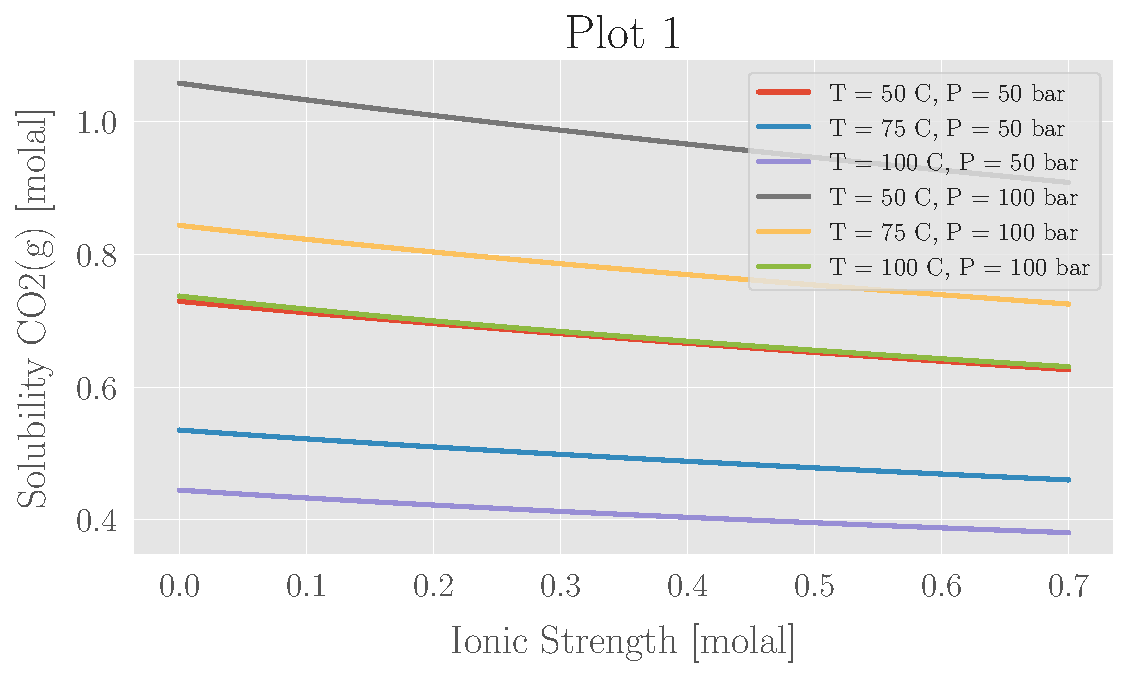
\includegraphics[height=0.25\textheight]{codes/results-useideal-0-userefpotentials-0/plot1-co2-solubility-vs-ionic-strength}}\\
\caption{Plot 1 performed for three different scenarios.}
\end{figure}

\begin{figure}
\centering
\subfloat[Performed\textbf{ without corrections} on the species activities,
$a_{i}$, and \textbf{ without interpolation} for the standard chemical
potentials, $\mu_{i}^{\circ}$.]{

\includegraphics[height=0.25\textheight]{codes/results-useideal-1-userefpotentials-1/plot2-co2-solubility-vs-temperature}}\\
\subfloat[Performed\textbf{ without corrections} on the species activities,
$a_{i}$, but\textbf{ with interpolation} for the standard chemical
potentials, $\mu_{i}^{\circ}$.]{

\includegraphics[height=0.25\textheight]{codes/results-useideal-1-userefpotentials-0/plot2-co2-solubility-vs-temperature}}\\
\subfloat[Performed\textbf{ with corrections} on the species activities, $a_{i}$,
and\textbf{ with interpolation} for the standard chemical potentials,
$\mu_{i}^{\circ}$.]{
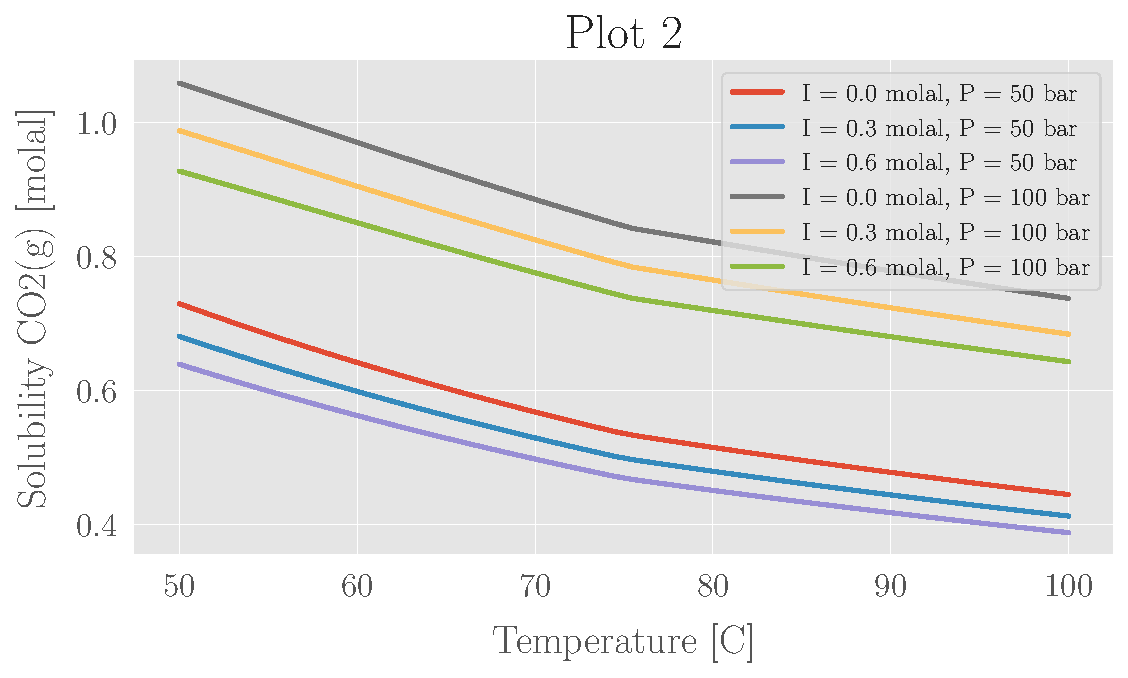
\includegraphics[height=0.25\textheight]{codes/results-useideal-0-userefpotentials-0/plot2-co2-solubility-vs-temperature}}
\caption{Plot 2 performed for three different scenarios.}
\end{figure}

\begin{figure}
\centering
\subfloat[Performed\textbf{ without corrections} on the species activities,
$a_{i}$, and\textbf{ without interpolation} for the standard chemical
potentials, $\mu_{i}^{\circ}$.]{

\includegraphics[height=0.25\textheight]{codes/results-useideal-1-userefpotentials-1/plot3-co2-solubility-vs-pressure}}\\
\subfloat[Performed\textbf{ without corrections} on the species activities,
$a_{i}$, but\textbf{ with interpolation} for the standard chemical
potentials, $\mu_{i}^{\circ}$.]{

\includegraphics[height=0.25\textheight]{codes/results-useideal-1-userefpotentials-0/plot3-co2-solubility-vs-pressure}}\\
\subfloat[Performed\textbf{ with corrections} on the species activities, $a_{i}$,
and\textbf{ with interpolation} for the standard chemical potentials,
$\mu_{i}^{\circ}$.]{
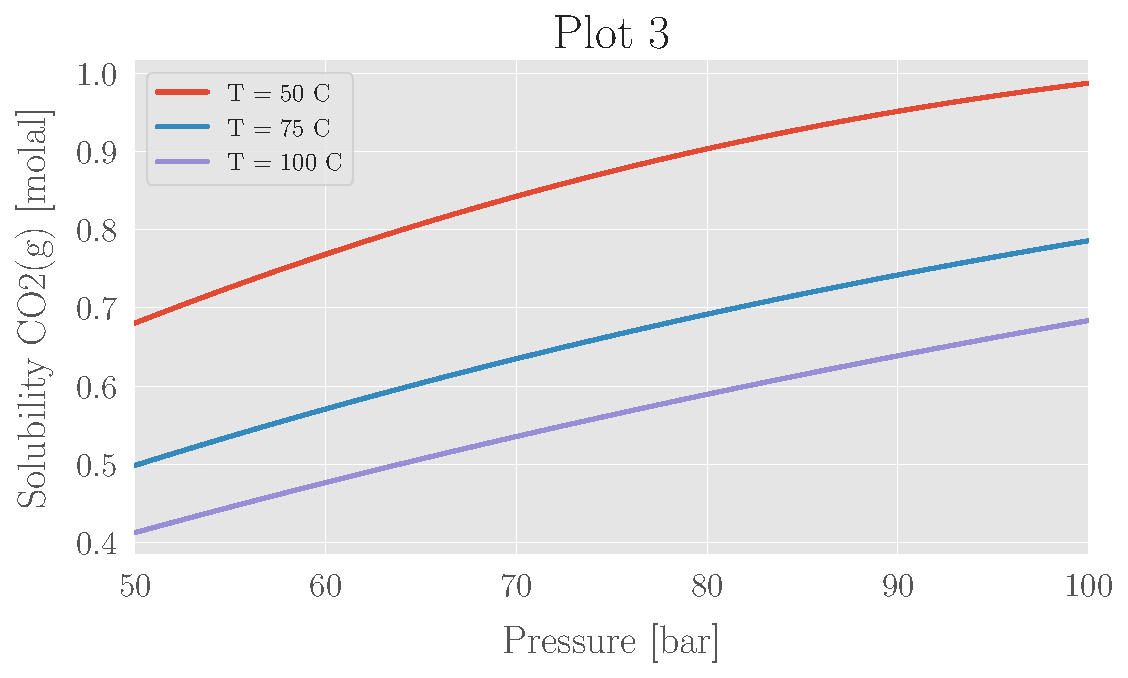
\includegraphics[height=0.25\textheight]{codes/results-useideal-0-userefpotentials-0/plot3-co2-solubility-vs-pressure}}
\caption{Plot 3 performed for three different scenarios.}
\end{figure}

\begin{figure}
	\centering
	\subfloat[Performed\textbf{ without corrections} on the species activities,
	$a_{i}$, and\textbf{ without interpolation} for the standard chemical
	potentials, $\mu_{i}^{\circ}$.]{
		
\includegraphics[height=0.25\textheight]{codes/results-useideal-1-userefpotentials-1/plot4-ph-vs-co2-amount}} \\
	\subfloat[Performed\textbf{ without corrections} on the species activities,
	$a_{i}$, but \textbf{ with interpolation} for the standard chemical
	potentials, $\mu_{i}^{\circ}$.]{
		
\includegraphics[height=0.25\textheight]{codes/results-useideal-1-userefpotentials-0/plot4-ph-vs-co2-amount}}\\
	\subfloat[Performed\textbf{ with corrections} on the species activities, $a_{i}$,
	and \textbf{ with interpolation} for the standard chemical potentials,
	$\mu_{i}^{\circ}$.]{
		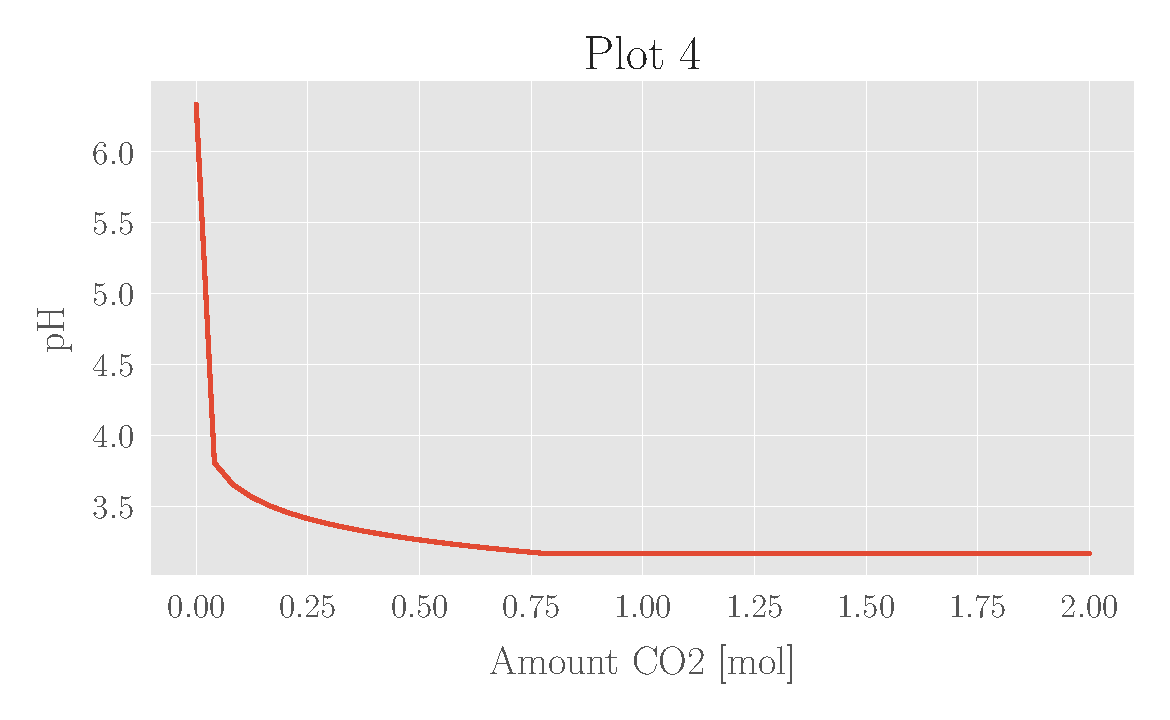
\includegraphics[height=0.25\textheight]{codes/results-useideal-0-userefpotentials-0/plot4-ph-vs-co2-amount}}
	\caption{Plot 4 performed for three different scenarios.}
\end{figure}

\begin{figure}
\centering
\subfloat[Performed\textbf{ without corrections} on the species activities,
$a_{i}$, and\textbf{ without interpolation} for the standard chemical
potentials, $\mu_{i}^{\circ}$.]{

\includegraphics[height=0.25\textheight]{codes/results-useideal-1-userefpotentials-1/plot5-calcite-solubility-vs-co2-amount}}\\
\subfloat[Performed\textbf{ without corrections} on the species activities,
$a_{i}$, but\textbf{ with interpolation} for the standard chemical
potentials, $\mu_{i}^{\circ}$.]{

\includegraphics[height=0.25\textheight]{codes/results-useideal-1-userefpotentials-0/plot5-calcite-solubility-vs-co2-amount}} \\
\subfloat[Performed\textbf{ with corrections} on the species activities, $a_{i}$,
and\textbf{ with interpolation} for the standard chemical potentials,
$\mu_{i}^{\circ}$.]{
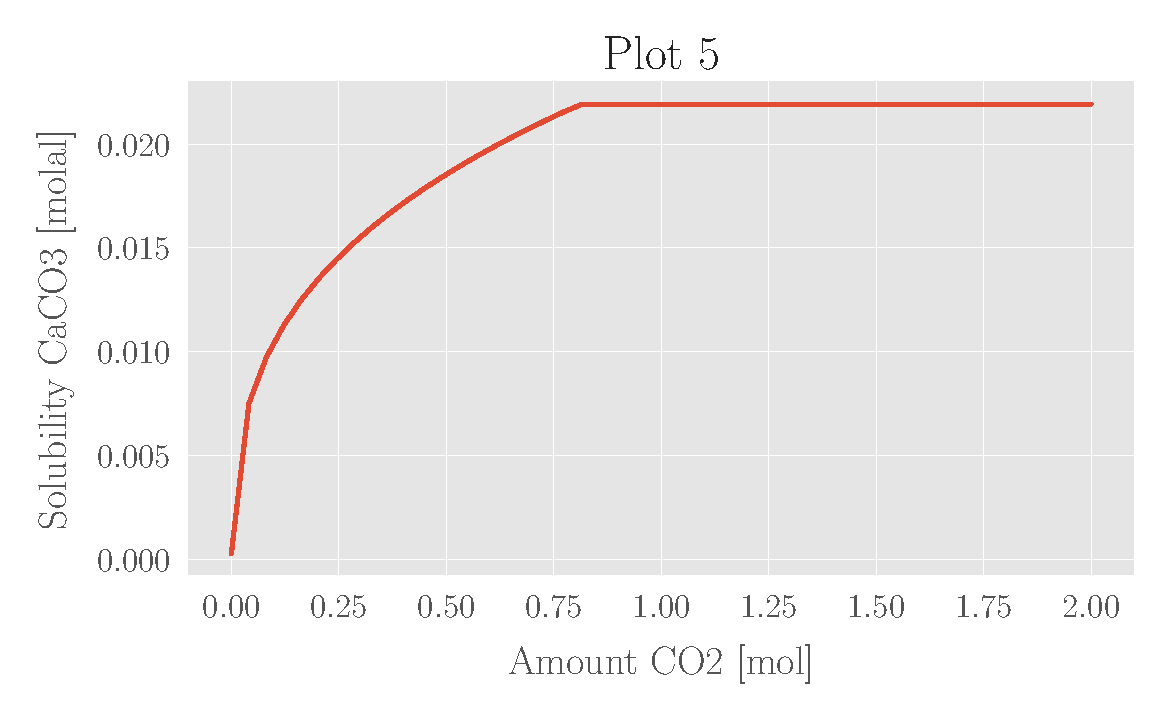
\includegraphics[height=0.25\textheight]{codes/results-useideal-0-userefpotentials-0/plot5-calcite-solubility-vs-co2-amount}}
\caption{Plot 5 performed for three different scenarios.}
\end{figure}

\begin{figure}
\centering
\subfloat[Performed\textbf{ without corrections} on the species activities,
$a_{i}$, and\textbf{ without interpolation} for the standard chemical
potentials, $\mu_{i}^{\circ}$.]{

\includegraphics[height=0.25\textheight]{codes/results-useideal-1-userefpotentials-1/plot6-calcite-solubility-mass-vs-co2-amount}} \\
\subfloat[Performed\textbf{ without corrections} on the species activities,
$a_{i}$, but\textbf{ with interpolation} for the standard chemical
potentials, $\mu_{i}^{\circ}$.]{

\includegraphics[height=0.25\textheight]{codes/results-useideal-1-userefpotentials-0/plot6-calcite-solubility-mass-vs-co2-amount}}\\
\subfloat[Performed\textbf{ with corrections} on the species activities, $a_{i}$,
and\textbf{ with interpolation} for the standard chemical potentials,
$\mu_{i}^{\circ}$.]{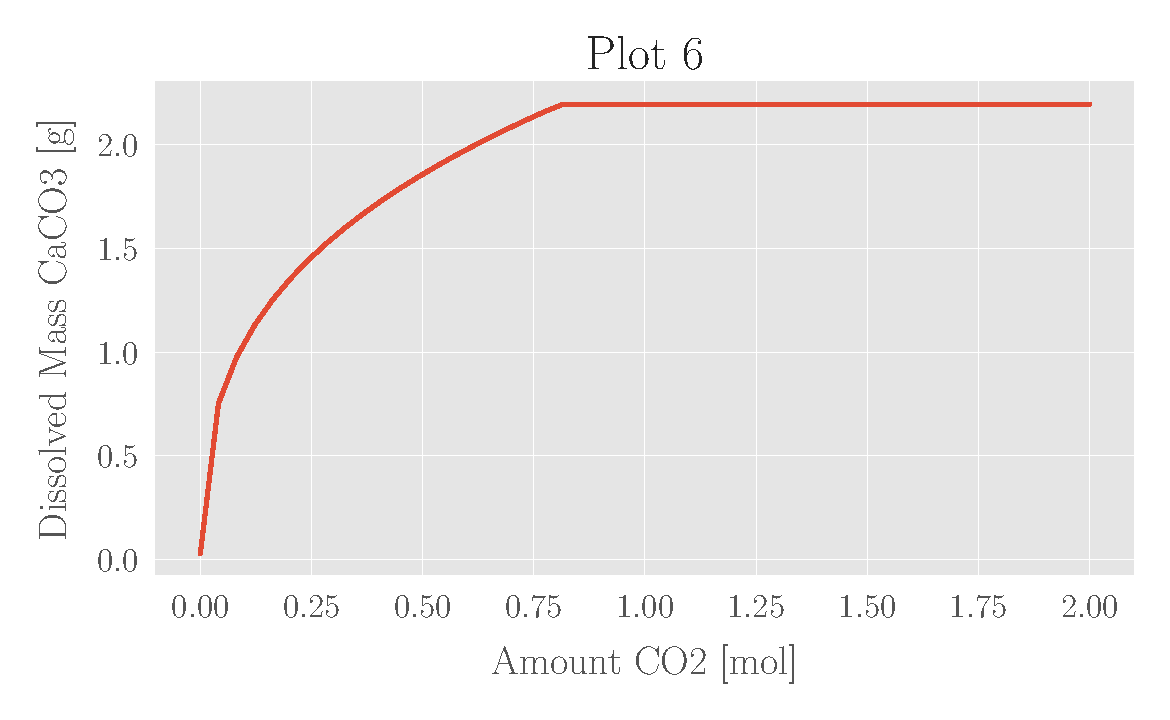
\includegraphics[height=0.25\textheight]{codes/results-useideal-0-userefpotentials-0/plot6-calcite-solubility-mass-vs-co2-amount}}
\caption{Plot 6 performed for three different scenarios.}
\end{figure}

\begin{figure}
	\centering
	\subfloat[Performed\textbf{ without corrections} on the species activities,
	$a_{i}$, and\textbf{ without interpolation} for the standard chemical
	potentials, $\mu_{i}^{\circ}$.]{
		
\includegraphics[height=0.25\textheight]{codes/results-useideal-1-userefpotentials-1/plot7-calcite-solubility-vs-ionic-strength}} \\
	\subfloat[Performed\textbf{ without corrections} on the species activities,
	$a_{i}$, but\textbf{ with interpolation} for the standard chemical
	potentials, $\mu_{i}^{\circ}$.]{
		
\includegraphics[height=0.25\textheight]{codes/results-useideal-1-userefpotentials-0/plot7-calcite-solubility-vs-ionic-strength}}\\
	\subfloat[Performed\textbf{ with corrections} on the species activities, $a_{i}$,
	and\textbf{ with interpolation} for the standard chemical potentials,
	$\mu_{i}^{\circ}$.]{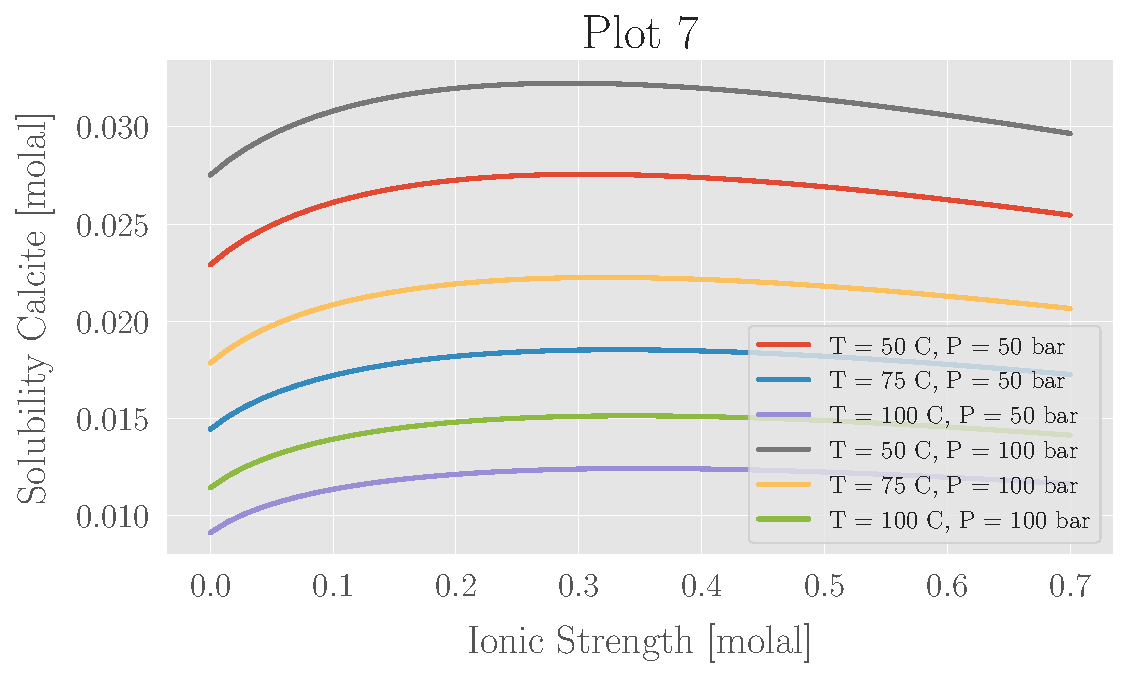
\includegraphics[height=0.25\textheight]{codes/results-useideal-0-userefpotentials-0/plot7-calcite-solubility-vs-ionic-strength}}
	\caption{Plot 7 performed for three different scenarios.}
\end{figure}

\begin{figure}
	\centering
	\subfloat[Performed\textbf{ without corrections} on the species activities,
	$a_{i}$, and\textbf{ without interpolation} for the standard chemical
	potentials, $\mu_{i}^{\circ}$.]{
		
\includegraphics[height=0.25\textheight]{codes/results-useideal-1-userefpotentials-1/plot8-calcite-solubility-vs-temperature}} \\
	\subfloat[Performed\textbf{ without corrections} on the species activities,
	$a_{i}$, but\textbf{ with interpolation} for the standard chemical
	potentials, $\mu_{i}^{\circ}$.]{
		
\includegraphics[height=0.25\textheight]{codes/results-useideal-1-userefpotentials-0/plot8-calcite-solubility-vs-temperature}}\\
	\subfloat[Performed\textbf{ with corrections} on the species activities, $a_{i}$,
	and\textbf{ with interpolation} for the standard chemical potentials,
	$\mu_{i}^{\circ}$.]{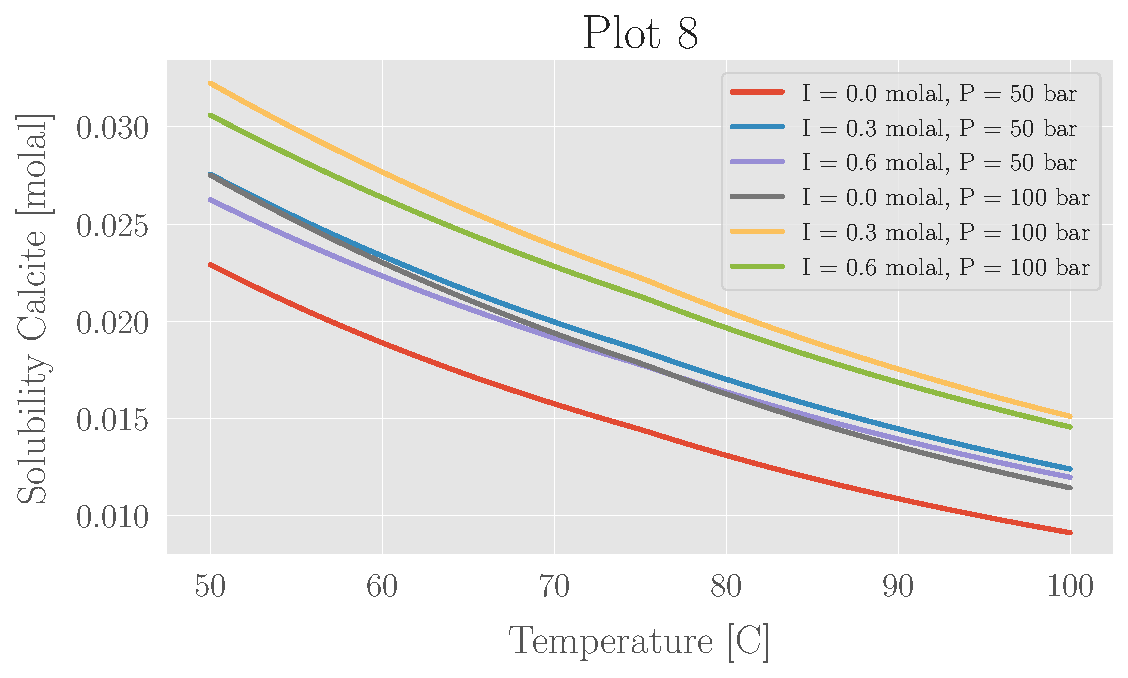
\includegraphics[height=0.25\textheight]{codes/results-useideal-0-userefpotentials-0/plot8-calcite-solubility-vs-temperature}}
	\caption{Plot 8 performed for three different scenarios.}
\end{figure}

\begin{figure}
	\centering
	\subfloat[Performed\textbf{ without corrections} on the species activities,
	$a_{i}$, and\textbf{ without interpolation} for the standard chemical
	potentials, $\mu_{i}^{\circ}$.]{
		
\includegraphics[height=0.25\textheight]{codes/results-useideal-1-userefpotentials-1/plot9-calcite-solubility-vs-pressure}} \\
	\subfloat[Performed\textbf{ without corrections} on the species activities,
	$a_{i}$, but\textbf{ with interpolation} for the standard chemical
	potentials, $\mu_{i}^{\circ}$.]{
		
\includegraphics[height=0.25\textheight]{codes/results-useideal-1-userefpotentials-0/plot9-calcite-solubility-vs-pressure}}\\
	\subfloat[Performed\textbf{ with corrections} on the species activities, $a_{i}$,
	and\textbf{ with interpolation} for the standard chemical potentials,
	$\mu_{i}^{\circ}$.]{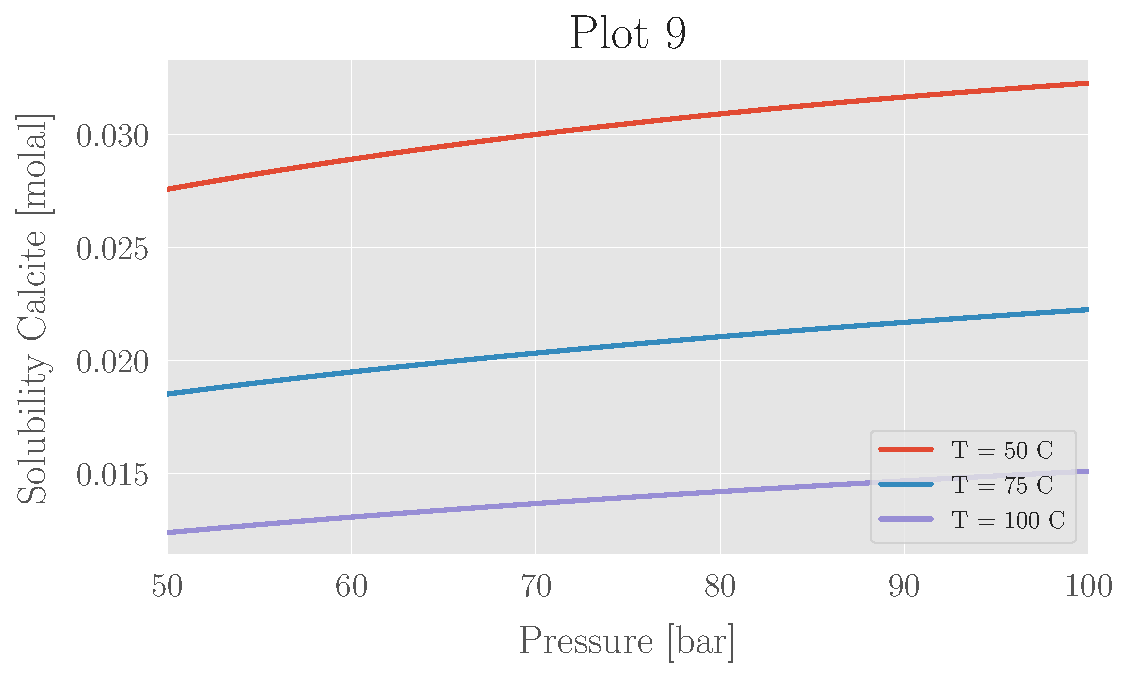
\includegraphics[height=0.25\textheight]{codes/results-useideal-0-userefpotentials-0/plot9-calcite-solubility-vs-pressure}}
	\caption{Plot 9 performed for three different scenarios.}
\end{figure}

\end{document}
